\chapter{Mapping BPMN to Jiac AgentBeans}
\label{chap:mapping}
The element mapping from BPMN to Jiac AgentBeans is created based on the existing mapping to JiacV - JADL script. In comparation to a JADL script, an AgentBean is written completely in Java, enabling more possibilities in mapping concepts such as intermediate Event handling. This chapter will provide a tabular overview of the mapping.\\\\
\textbf{\large{Business Process Diagram}}\\
		\begin{tabularx}{\linewidth}{|l|X|}\hline\hline
			\multicolumn{2}{|c|}{\textbf{Business Process Diagram}} \\\hline\hline
			 Pool & A pool is currently mapped to an Agent Bean extending the AbstractMethodExposingBean. The name of the bean is derived from the pool name and the name of the business process diagram it is contained in.\\
			 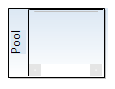
\includegraphics{images/mapping/pool.png}  & 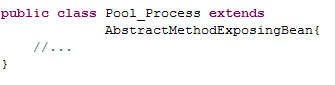
\includegraphics{images/mapping/poolcode.png}\\\hline
			 \end{tabularx}\\\\
			 
			 
		\begin{tabularx}{\linewidth}{|l|X|}\hline\hline
			 Process & The process content in a pool is mapped to a Workflow Method in the generated AgentBean. Depending on the type of the StartEvent, an Action might be exposed, enabling this method to be invoked as a service. This method will contain a Script which is generated from the flowObjects contained in the process.\\
			 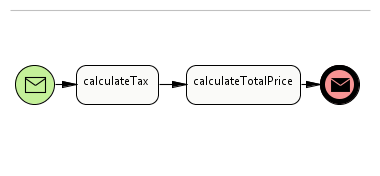
\includegraphics[width=0.3\textwidth]{images/mapping/process.png}  & 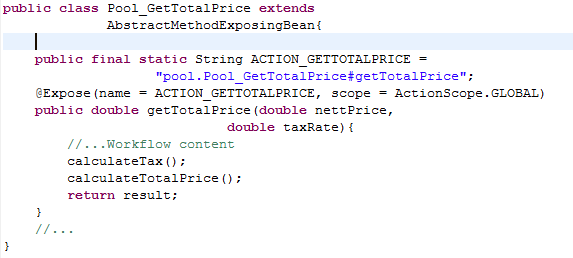
\includegraphics[width=0.7\textwidth]{images/mapping/processcode.png}\\\hline
			 Lane & Lanes will not be mapped in this mapping\\\hline \hline
		\end{tabularx}\\\\
%%%%%%%%%%%%%%%%%%%%%%%%%%%%%%%%%%%
% Events                          %
%%%%%%%%%%%%%%%%%%%%%%%%%%%%%%%%%%%				
\textbf{\Large{Events}}\\\\
For intermediate Events, an EventHandlerThread will be generated and started. If the intermediate Event is attached to an activity, the activity will also be started as a Thread. 

		\begin{tabularx}{\linewidth}{|l|X|}\hline\hline
			\multicolumn{2}{|c|}{\textbf{Start Events}} \\\hline\hline
			 Timer & The generated process will be started in the execute() method of the JIAC AgentBean\\\hline
			 Message & If the implementation is a Service, an action will be created, and the process can be started through a service call (invoke). If the implementation is a Message Channel, a Space Observer will be attached to the agents memory, and the process will start as soon as a message is recieved.\\\hline
			 Rule & Rule start events are not regarded in the current mapping\\\hline
			 Link & \\\hline
			 Multiple & If a pool has multiple start events, each start event will be mapped according to it's respective trigger\\\hline\hline
			 
			 \multicolumn{2}{|c|}{\textbf{Intermediate Events}} \\\hline\hline
			 Rule & not regarded in the current mapping\\\hline
			 Timer & A TimerEventHandler will be created and started.\\\hline
			 Message & A MessageEventHandler will be created and started. \\\hline
			 Link & ...\\\hline
			 Multiple & each event will be mapped according to it's respective trigger\\\hline
			 Cancel & ... \\\hline
			 Compensate & ... \\\hline
			 Error & If attached to an activity, the method generated from the activity will be called in a try-catch block \\\hline\hline
			 
			 \multicolumn{2}{|c|}{\textbf{End Events}} \\\hline\hline
			 Message & If implementation is Message Channel, a message with the payload will be written to the channel \\\hline
			 Link & \\\hline
			 Multiple & \\\hline
			 Cancel & \\\hline
			 Compensate & \\\hline
			 Error & The generated service will throw an exception\\\hline
			 Terminate & \\\hline
		\end{tabularx}\\\\

\textbf{\large{Activities}}\\\\
Basically, an Activity-method will be created for each activity, and then a script calling this method will be added into the Workflow-method. This way, each activity can have their own scope of variables. 
	
		\begin{tabularx}{\linewidth}{|l|X|}\hline\hline
			\multicolumn{2}{|c|}{\textbf{Activity}}\\\hline\hline
			 Standard Loop & ... \\\hline
			 Multi Instance Loop & ... \\\hline
			 With Event Handler & the method generated will be started parallel to an EventHandlerThread. When the activity is completed, the EventHandlerThread will be terminated. In contrary, if the Event is trigerred before the activity is completed, the Thread performing the activity will be interrupted. \\\hline\hline	
				\multicolumn{2}{|c|}{\textbf{Task}}\\\hline\hline
					Manual & manual task will be ignored\\\hline
			 		Recieve & ...\\\hline
			 		Send & ...\\\hline
			 		Service & service tasks will be mapped into a service call(invoke)\\\hline
					Script & the given script will be added into the activity method. The script has to be written in java or the resulting code will have syntax error(not checked)\\\hline
			 		Reference & ... \\\hline
			 		User & ...\\\hline\hline
			 \multicolumn{2}{|c|}{\textbf{Subprocess}} \\\hline\hline
			 		Embedded & \\\hline
			 		Reference & \\\hline
					Independent & \\\hline
					Transaction & \\\hline\hline
		\end{tabularx}\\\\
		
	\textbf{\Large{Gateways}}\\\\
		\begin{tabularx}{\linewidth}{|l|X|}\hline\hline
		\multicolumn{2}{|c|}{\textbf{Gateway}}\\\hline\hline
		XOR Data(Loop) & \\\hline
		XOR Data(Block) & \\\hline
		XOR Event & \\\hline
		AND & Each branch will be wrapped in a paralel execution\\\hline
		OR & \\\hline
		COMPLEX & \\\hline\hline
		\end{tabularx}\\\\
		
	\textbf{\Large{Other Elements}}\\\\
		\begin{tabularx}{\linewidth}{|l|X|}\hline\hline
		\multicolumn{2}{|c|}{\textbf{Connections}}\\\hline\hline
		Sequence Flow & \\\hline
		Message Flow& \\\hline
		Association & \\\hline\hline
		\multicolumn{2}{|c|}{\textbf{Artifact}}\\\hline\hline
		Data Object & \\\hline
		Text Annotation & text annotations can be added as a comment block in the code \\\hline
		Group & \\\hline
		Custom Artifact & \\\hline
		\end{tabularx}\\\\